\lab{Importance Sampling and Monte Carlo Simulations}{Importance Sampling and Monte Carlo Simulations}
\objective{Use importance sampling to reduce the error and variance of Monte Carlo Simulations.}
\label{lab:montecarlo2}

\section*{Introduction}

Using the traditional methods of Monte Carlo integration as discussed in the previous lab are not always the most efficient means to estimate an integral. For example, assume we were trying to find the probability that a randomly chosen variable $Y$ from the standard normal distribution is greater than $3$. We know that one way to solve this by solving the following integral:

\begin{equation} \label{eq:integral} 
P(Y > 3) = \int_{3}^{\infty} f_X(t) dt = \frac{1}{\sqrt{2\pi}}\int_{3}^{\infty} e^{-t^2/2} dt
\end{equation}
By the Law of the Unconscious Statistician, we can restate the integral above as

\begin{equation*}
\int_{3}^{\infty} f_X(t) dt = \int_{-\infty}^{\infty} h(t)f_X(t) dt = E[h(X);f_X]
\end{equation*}
where $E[h(X);f_X]$ refers to the expected value of $h(X)$ with the random variable $X$ being generated by $f_X$, and where

$$h(t) = \begin{cases}
1 & \text{ if } t > 3 \\ 
0 & \text{ if } t \leq 3 
\end{cases} $$

\section*{Monte Carlo Simulation}
We can estimate this same probabilty using Monte Carlo simulation. 
Given a random i.i.d. sample $x_1, x_2, \cdots , x_N$ generated by $f_X$, we can estimate $E[h(X);f_X]$ using
\begin{equation} \label{eq:estimator}
\widehat{E}_n[h(X);f_X] = \frac{1}{N}\sum_{i = 1}^{N}h(x_i)
\end{equation}

Now that we have defined the estimator, it is now quite manageable to approximate Equation \ref{eq:integral}. By the Weak Law of Large Numbers, the estimate will get closer and closer to the actual value as we use more and more sample points.

\begin{comment}
\begin{lstlisting}
>>> h = lambda x : x > 3
>>> N = 10**7
>>> x = np.random.normal(size=N)
>>> 1./N * np.sum(h(x))
0.0013644
\end{lstlisting}
\end{comment}

\begin{problem} \label{prob:mc}
Write a function in Python that estimates the probability that a random draw from the standard normal distribution is greater than 3 using Equation \ref{eq:estimator}. Your answer should approach $0.0013499$ for sufficiently large samples. What estimate do you get when you use a sample with $10^7$ points?
\end{problem}

Though this approach gets the job done, it turns out that this isn't very efficient. Since the probability of drawing a number greater than $3$ from the standard normal distribution is so unlikely, it turns out we need many sample points to get a good approximation.

\section*{Importance Sampling}
Importance sampling is one way to make Monte Carlo simulations converge much faster. We chose a different distribution to sample our points to generate more \emph{important} points. With our example, we want to choose a distribution that would generate more numbers around 3 to get a more reliable estimate. The theory behind importance sampling boils down to the following result:
\begin{equation} \label{eq:importance}
\begin{split}
E[h(X);f_X] & = \int_{-\infty}^{\infty} h(t)f_X(t) dt \\
& = \int_{-\infty}^{\infty} h(t)f_X(t)\left ( \frac{g_X(t)}{g_X(t)} \right ) dt \\
& = \int_{-\infty}^{\infty} \left ( \frac{h(t)f_X(t)}{g_X(t)} \right )g_X(t) dt \\
& = E\left [ \frac{h(X)f_X(X)}{g_X(X)} ; g_X \right ]
\end{split}
\end{equation}

The corresponding estimator is,

\begin{equation*}
\begin{split}
\widehat{E}[h(X);f_X] & = \widehat{E}\left [ \frac{h(X)f_X(X)}{g_X(X)} ; g_X \right ] \\
& = \frac{1}{N}\sum_{i = 1}^{N}\frac{h(x_i)f(x_i)}{g_X(x_i)}
\end{split}
\end{equation*}

The function $f_X$ is the p.d.f of the \emph{target distribution}. The function $g_X$ is the p.d.f of the \emph{importance distribution}. The fraction $\frac{f_X(X)}{g_X(X)}$ is called the \emph{importance weight}. This allows us to draw a sample from any distribution as long as we multiply $h(X)$ by the likelihood ratio. We will solve the same problem as in Problem \ref{prob:mc} using importance sampling. We will choose $g_X$ to be the normal distribution with $\mu = 4$ and $\sigma = 1$. We have chosen this distribution because it will give us more points closer to and greater than 3.

\begin{lstlisting}
>>> import scipy.stats as ss
>>> f = lambda x : x > 3
>>> h = lambda x : ss.norm().pdf(x)
>>> g = lambda x : ss.norm(loc=4,scale=1).pdf(x)

# Sample from the N(4,1).
>>> N = 10**7
>>> X = np.random.normal(4,scale=1,size=N)

# Calculate estimate.
>>> 1./N * np.sum(f(X)*h(X)/g(X))
0.00134921134631
\end{lstlisting}

\begin{figure}[H]
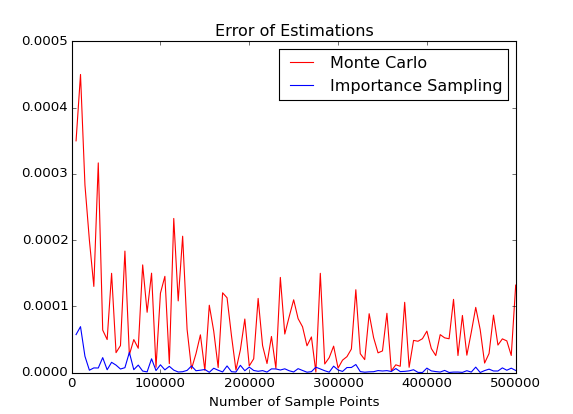
\includegraphics[width=\textwidth]{MCvsIS.png}
\caption{Comparison of error between standard method Monte Carlo and Importance Sampling method of Monte Carlo.}
\label{fig:compare}
\end{figure}

\begin{problem} \label{prob:gamma}
A tech support hotline receives an average of 2 calls per minute. What is the probability that they will have to wait at least 10 minutes to receive 9 calls? Implement your estimator using importance sampling. Calculate estimates using 5000, 10000, 15000, $\cdots$, 500000 sample points. Your answers should approach $0.00208725$.

Hint: The version of the gamma distribution is \li{scipy.stats} is determined by the shape and the scale ($\theta$) of the distribution. You may be used to the gamma distribution being defined in terms of the shape and the rate ($\beta$). You can remedy this with the fact that $\theta = 1/\beta$.
\end{problem}

\begin{problem}
In this problem, we will visualize the benefits of importance sampling. Create a plot of the error of the traditional methods of Monte Carlo and the importance sampling methods of Monte Carlo. What do you observe? Your answers should resemble Figure \ref{fig:compare}.

Hint: The following code solves Problem \ref{prob:gamma} using traditional methods of Monte Carlo:
\begin{lstlisting}
h = lambda x : x > 10
MC_estimates = []
for n in xrange(5000,505000,5000):
    X = np.random.gamma(9,scale=0.5,size=N)
    MC = 1./N*np.sum(h(X))    
    MC_estimates.append(MC)
MC_estimates = np.array(MC_estimates)
\end{lstlisting}

Hint: The following code returns the actual value of Equation \ref{eq:integral}:
\begin{lstlisting}
1 - ss.gamma(a=9,scale=0.5).cdf(10)
\end{lstlisting}
\end{problem}

\section*{Generalizing the Principles of Importance Sampling}
The examples we have explored to this point in the lab were merely educational. Since we have a simple means of calculating the correct answer to Problem \ref{prob:gamma}, it doesn't make much sense to use methods of Monte Carlo in this situation. However, as discussed in the previous lab, there are not always closed-form solutions to the integrals we want to compute.

We can extend the same principles we have discussed thusfar to solve many types of problems. For a more general problem, we can implement importance sampling by doing the following:
\begin{enumerate}
\item Define a function $h$ where, $h(t) = \begin{cases}
1 & \text{ if condition is met }  \\ 
0 & \text{ otherwise}
\end{cases} $.  
\item Define a function $f_X$ which is the p.d.f. of the target distribution. 
\item Define a function $g_X$ which is the p.d.f. of the importance distribution.
\end{enumerate}

\begin{problem}
The joint normal distribution of $N$ independent random variables with mean 0 and variance 1 is
\[
f_X(\x) = \frac{1}{\sqrt{(2 \pi)^N}} e^{-(\x^T\x)/2}.
\]
The integral of $f_X(\x)$ over a box is the probability that a draw from the distribution will be in the box.
However, $f_X(\x)$ does not have a symbolic antiderivative.


\begin{comment}
\item The integral of this function on $B = [-1,1]\times [-1,1]\times[-1,1] \subset \mathbb{R}^3$ can be computed in SciPy with the following code.
\begin{lstlisting}
>>> import scipy.stats as stats

# Define the bounds of the box to integrate over
>>> mins = np.array([-1, -1, -1])
>>> maxs = np.array([1, 1, 1])

# Each variable has mean 0
>>> means = np.zeros(3)

# The covariance matrix of N independent random variables
#    is the NxN identity matrix.
>>> covs = np.eye(3)

# Compute the integral
>>> value, inform = stats.mvn.mvnun(mins, maxs, means, covs)
\end{lstlisting}
Then \li{value} is the integral of $f(\x)$ on $B$.
Use SciPy to integrate $f(\x)$ on $\Omega=[-0.5, 0.75]\times[0,1]\times[0, 0.5]\times[0,1] \subset \mathbb{R}^4$.
\end{comment}

Use what you have learned about importance sampling to estimate the probability that a given random variable in $\mathbb{R}^2$ generated by $f_X$ will be less than -1.75 in the x-direction and greater than 1.25 in the y-direction.

Treat $f_X$ as the p.d.f. of your target distribution.
Use the function \li{stats.multivariate_normal} to create a multivariate normal distribution to serve as your importance distribution. 
This function accepts a numpy array \li{mean} and a numpy array \li{cov}. 
The parameter \li{mean} is an array of the mean of each direction. 
The parameter \li{cov} is the covariance matrix. 
In this case, the covariance matrix will be a diagonal matrix with the variance of each variable down the diagonal. 

\end{problem}

\section*{Unnormalized Target Densities}
The methods discussed so far are only applicable if the target density is normalized, or in other words, has an integral of 1. If the target density is not normalized, Equation \ref{eq:importance} becomes,

\begin{equation*} \label{eq:unnormalized}
\begin{split}
E[h(X);f] & = \frac{\int h(t)f(t) dt}{\int f(t) dt} \\
& = \frac{\int h(t)f(t) \left ( \frac{g_X(t)}{g_X(t)} \right ) dt}{{\int f(t)} \left ( \frac{g_X(t)}{g_X(t)} \right ) dt} \\
& = \frac{\int \left ( \frac{h(t)f(t)}{g_X(t)} \right ) g_X(t) dt}{\int \left ( \frac{f(t)}{g_X(t)} \right ) g_X(t) dt} \\
& = \frac{E\left [ \frac{h(X)f(X)}{g_X(X)} ; g_X \right ]}{E\left [ \frac{f(X)}{g_X(X)} ; g_X \right ]}
\end{split}
\end{equation*}

The corresponding estimator becomes,
\begin{equation*}
\begin{split}
\widehat{E}_n[h(X);f] & = \frac{E\left [ \frac{h(X)f(X)}{g_X(X)} ; g_X \right ]}{E\left [ \frac{f(X)}{g_X(X)} ; g_X \right ]} \\
& = \frac{\frac{1}{N}\sum_{i = 1}^{N}\frac{h(x_i)f(x_i)}{g_X(x_i)}}{\frac{1}{N}\sum_{i = 1}^{N}\frac{f(x_i)}{g_X(x_i)}} \\
\end{split}
\end{equation*}
